% $Id: template.tex 11 2007-04-03 22:25:53Z jpeltier $
% TODO:
% check citations are correct: like one space after them?
% have people estimate distances?/ tour people around
% widespread use, it has to be comfortable
% people have to be able to use their arms while doing

\documentclass{vgtc}                          % final (conference style)
% \documentclass[review]{vgtc}                 % review
% \documentclass[widereview]{vgtc}             % wide-spaced review
% \documentclass[preprint]{vgtc}               % preprint
% \documentclass[electronic]{vgtc}             % electronic version

%% Uncomment one of the lines above depending on where your paper is
%% in the conference process. ``review'' and ``widereview'' are for review
%% submission, ``preprint'' is for pre-publication, and the final version
%% doesn't use a specific qualifier. Further, ``electronic'' includes
%% hyperreferences for more convenient online viewing.

%% Please use one of the ``review'' options in combination with the
%% assigned online id (see below) ONLY if your paper uses a double blind
%% review process. Some conferences, like IEEE Vis and InfoVis, have NOT
%% in the past.

%% Figures should be in CMYK or Grey scale format, otherwise, colour 
%% shifting may occur during the printing process.

%% These three lines bring in essential packages: ``mathptmx'' for Type 1 
%% typefaces, ``graphicx'' for inclusion of EPS figures. and ``times''
%% for proper handling of the times font family.

\usepackage{graphicx}
\usepackage{mathptmx}
\usepackage{times}

%% We encourage the use of mathptmx for consistent usage of times font
%% throughout the proceedings. However, if you encounter conflicts
%% with other math-related packages, you may want to disable it.

%% If you are submitting a paper to a conference for review with a double
%% blind reviewing process, please replace the value ``0'' below with your
%% OnlineID. Otherwise, you may safely leave it at ``0''.
\onlineid{0}

%% declare the category of your paper, only shown in review mode
\vgtccategory{Research}

%% allow for this line if you want the electronic option to work properly
\vgtcinsertpkg

%% In preprint mode you may define your own headline.
% \preprinttext{To appear in an IEEE VGTC sponsored conference.}

%% Paper title.

\title{Utilizing Myo Armbands for Various Locomotion Methods}

%% This is how authors are specified in the conference style

%% Author and Affiliation (single author).
%% \author{Roy G. Biv\thanks{e-mail: roy.g.biv@aol.com}}
%% \affiliation{\scriptsize Allied Widgets Research}

%% Author and Affiliation (multiple authors with single affiliations).
%% \author{Roy G. Biv\thanks{e-mail: roy.g.biv@aol.com} %
%% \and Ed Grimley\thanks{e-mail:ed.grimley@aol.com} %
%% \and Martha Stewart\thanks{e-mail:martha.stewart@marthastewart.com}}
%% \affiliation{\scriptsize Martha Stewart Enterprises \\ Microsoft Research}

%% Author and Affiliation (multiple authors with multiple affiliations)
\author{Preston TunneLL WiLson\\ %
  \scriptsize Rhodes CoLLege %
  \and Ansel MaclaughLin\\ %
  \scriptsize Rhodes College %
  \and WiLL KaLescky\\ %
  \scriptsize{Rhodes CoLLege}%
  \and Betsy WiLLiams\thanks{sandersb@rhodes.edu}\\ %
  \scriptsize Rhodes CoLLege}

%% A teaser figure can be included as follows, but is not recommended since
%% the space is now taken up by a full width abstract.
% \teaser{
% 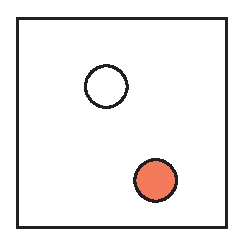
\includegraphics[width=1.5in]{sample.eps}
% \caption{Lookit! Lookit!}
% }

%%   Abstract section.
%\abstract{
%  In this paper, we use the Myo armband, an inexpensive wearable device (199 USD),
%  to implement a suite of locomotion algorithms.
%  This expands upon our previous work implementing a single arm swing navigation method\cite{previousMYO}.
%  We are in the pilot stage of this experiment,
%  but we plan to compare each locomotion method to
%  joystick locomotion and physical walking using a spatial orientation task.
%  We have selected the Myo as the basis of our navigation methods
%  as it is inexpensive compared to tracking systems that permit foot exploration,
%  does not suffer from space constraints,
%  and requires less physical energy than walking on foot.
%  Additionally, we have found it to be more precise and accurate than our previous Microsoft Kinect WIP algorithms.
%} % end of abstract

%% ACM Computing Classification System (CCS). 
%% See <http://www.acm.org/class/1998/> for details.
%% The ``\CCScat'' command takes four arguments.

\CCScatlist{ 
  %\CCScat{H.5.1}{Multimedia Information Systems}{Artificial, augmented, and virtual realities};
  \CCScat{I.3.7}{Computer Graphics}{Three-Dimensional Graphics and Realism}{Virtual reality}
}

%% Copyright space is enabled by default as required by guidelines.
%% It is disabled by the 'review' option or via the following command:
% \nocopyrightspace

%%%%%%%%%%%%%%%%%%%%%%%%%%%%%%%%%%%%%%%%%%%%%%%%%%%%%%%%%%%%%%%% 
%%%%%%%%%%%%%%%%%%%%%% START OF THE PAPER %%%%%%%%%%%%%%%%%%%%%%
%%%%%%%%%%%%%%%%%%%%%%%%%%%%%%%%%%%%%%%%%%%%%%%%%%%%%%%%%%%%%%%%% 

\begin{document}

%% The ``\maketitle'' command must be the first command after the
%% ``\begin{document}'' command. It prepares and prints the title block.

%%   the only exception to this rule is the \firstsection command
\firstsection{Introduction}

\maketitle

%% \section{Introduction} 
Two inexpensive methods of exploring a virtual environment are ``walking in place'' (WIP) and arm swinging.
These techniques are compelling because they seem to provide more proprioceptive cues than traditional inexpensive virtual navigation techniques like a joystick.
More specifically, WIP and arm swinging seem to result in better spatial awareness of the environment.
For example, in our prior work, we had success in implementing a WIP method using an inexpensive Nintendo Wii Balance Board \cite{Williams:2011:EWP} and later with Microsoft Kinect sensors \cite{Wilson:2014}.
We showed that participants' spatial orientation was the same as normal walking and superior to joystick navigation \cite{Williams:2011:EWP}.
We use an inexpensive wearable device called the Myo armband (199 USD) to implement a simple arm swinging algorithm that allows a user to freely explore an HMD-based virtual environment \cite{previousMYO}.
We found that our arm swinging method outperforms a simple joystick and that spatial orientation is comparable to physically walking on foot \cite{previousMYO}.


The purpose of this poster is two present two different navigation techniques using the Myo armband and evaluate them.
The Myo armband is a wearable device mounted with tracking devices as seen in Figure \ref{fig:morgan}.
First, we describe a walking in place algorithm that is implemented using a Myo worn around the ankle of the foot.
We believe that this method of implementing walking in place is more robust and simpler to implement than our previous algorithms \cite{Williams:2011:EWP,Wilson:2014}.
We plan to directly compare the Myo walking in place algorithm to Myo arm swinging using a spatial orientation task and usability rating.
Second, much of the work on navigation in virtual environments has focused on exploring a space while physically standing.
However, in this work, we developed a method of arm swinging using the Myo armband that allows the user to explore a space while physically sitting down.
We will examine spatial orientation as a user navigates using this method by directly comparing it to seated joystick exploration.



\section{Myo Implementation}
% TODO
% continue working on this
\begin{figure}[h]
  \centering
  \def\svgwidth{.2\textwidth}
  \input{morgan_and_myo.eps_tex}
  \caption{User wearing a Myo armband}
  \label{fig:morgan}
\end{figure}
The Myo armband is a wearable band (seen in Figure \ref{fig:morgan}).
To use our arm swinging method, subjects wear the Myo armband on the thickest part of their forearm, just below their elbow.
The armband is adjusted so that it fits comfortably snug, not sliding on the users’ arms when they move.
The armband fits arm sizes between 7.5in and 13in in circumference
by adding or removing the expanders that come with the product.
The Myo armband has two types of sensors:
medical grade stainless EMG sensors
and a 9 axis inertial internal measurement unit (IMU).
The IMU contains a three-axis gyroscope, a three-axis accelerometer, and a three-axis magnetometer.
Thus, the Myo SDK provides several kinds of spatial data: orientation in terms of pitch, yaw and roll;
acceleration vector data which represents the acceleration of the armband;
and angular velocity data provided by the gyroscope.
It is important to note that the IMU in the Myo armband can accurately measure the orientation of the arm (roll, pitch, yaw)
but position data has a significant amount of error.
The Myo armband is better suited for getting the relative orientations of the arms rather than the
absolute position of the arms.
It can achieve a sampling rate of 50 Hz.
All data from the Myo is communicated via Bluetooth to a computer.
Participants wore the armband
with the Myo logo facing directly outward when their arms were
at their side them as seen in Figure \ref{fig:morgan}.
As a result, the orientation sensor on the device is oriented to everyone’s arm in similar way.
It is important to note that we only used one Myo armband to implement this algorithm,
though we told the subjects to use both arms to move around in the IVE
when we were explaining the locomotion method.
This approximation works well because when one arm is swinging the other arm usually swings too.
To stop moving, participants stopped moving their arms.
With this arm swinging algorithm, if subjects swing their arms faster, they can propel themselves forward faster.

% full steps, occlusion, uncomfortable
In our previous work \cite{Wilson:2014}, we found some problems with using the Microsoft Kinect as the basis
of our navigation method in a virtual system.
The most immediate trouble was that there was occlusion of body parts:
when the user was facing certain orientations,
the Kinect would not be able to correctly determine the user's skeletal data.
We tried to remedy this by adding an additional Kinect to our system,
but this did not completely solve the problem.
To prevent the faulty Kinect data from causing users to shift forward unintentionally,
we increased the angle of the inner knee necessary to record a step.
This forced the users to practically march.
Users found this to be uncomfortable, while the experimenters found it to be funny.
Finally, users could only move forward in full step increments--users did not have precise control over their movement.

As we have previously had success with WIP \cite{Williams:2011:EWP},
we try to use the reliable and precise Myo base to create an inexpensive WIP system.
% Our novel approach presented in this work allows the user to walk in place with Myo.
% easier to implement;
This system is easier to implement.
Using two Kinects required that we set up a virtual private network to send skeletal data from both Kinects
to the computer running the environment.
Myo armbands use Bluetooth--even if we were to use multiple bands,
a single computer would be able to receive all of the information.
Similarly, we do not need to process two sets of data.
As the EMG sensors of the Myo armbands are designed for the user's arm,
the EMG data gathered from the leg will be useless.
We instead rely on the accelerometer data.
We simply measure the change in velocity from the Myo armband.
Users are able to walk in a way which is most comfortable to them rather than march.

%more robust, more precise
The Myo armband avoids the problem of occlusion faced by the Kinect.
No optical data is needed as data is read directly from the skin of the user.
Additionally, as we use the data from the accelerometer,
users have more precise control over their movement.
The faster they walk in place, the faster they move in the VE.
They can quickly stop and move slightly and comfortably.

Seated arm swinging is implemented similarly to our previous work \cite{previousMYO}.
%If we have time, we will improve our previous arm swinging method by only translating the user forward when
%they swing their arms forward.


\section{Experiment}
We intend to conduct two different experiments.
In Experiment 1,  we compare Myo WIP to our previous Myo arm swinging algorithm.
In Experiment 2, we compare arm swinging while seated to seated joystick navigation.
In both experiments the methodology will be identical.
More specifically, we plan to test subjects on their spatial orientation in the environment using within subject design.
In both conditions, we will test the users' spatial orientation by asking them to learn the layout of objects within the IVE.
We will then ask them to walk to a new location, close their eyes and turn to face a specified target.
Latency will be measured from the time the target is identified
until subjects say that they have completed their turning movement and are facing the target.
Turning errors will be measured as the difference between the direction the user is facing and the correct facing direction.



\section{Discussion}
% sell why these two experiments we are doing are good: comfortable and possible to be used widespread
Our previous experiment \cite{previousMYO} with the Myo armband shows that although the
proprioceptive cues of the arm swinging method do not exactly match physical walking,
the cyclic repetition of movement is similar to walking,
and humans swing their arms when they walk.
Moreover, Zehr et al. \cite{zehr} point out that both the arms and legs are coordinated by central pattern generators (CPG),
which are biological neural networks that produce rhythmic patterned outputs without sensory feedback.
Thus, arm and leg movements are regulated
by CPG activity and sensory feedback.
They also explain that the
strength of coupling between the legs is stronger than that between the arms.
Thus, we intend to expand the Myo algorithm to include walking in place locomotion. 
We hypothesize that the arm and leg movements prime the sensory motor system to process optical flow.
This idea of the movement condition priming the sensory motor system is consistent with
the literature \cite{Engel:2008VRST,Nitzsche2004:Presence,Razzaque2001:Eurographics,Steinicke:2010,Williams2006:APGV}.
Additionally, researchers \cite{Engel:2008VRST,Nitzsche2004:Presence,Razzaque2001:Eurographics,Steinicke:2010}
have previously designed an algorithm
that imperceptibly rotates the virtual environment so that the physical locomotion of the user fits within the
confines of the tracking system.
Again, researchers are able to successfully manipulate the mapping between normal physical walking
and visual flow in such a way that spatial orientation is maintained.
This provides the user with an opportunity to explore a virtual space
larger than the tracking space of the HMD.

%%SCIENCE ABOVE

We believe that our new Myo navigation methods, just as our previous one, will be superior to joystick locomotion because
users have difficulty mapping optical flow to pushing forward on a joystick since the act of holding onto a joystick could
itself be distracting.
In line with our prior WIP research, our current work and arm swing studies suggest that physical motion and cyclic action add
value to users' spatial updating.

We hypothesize that the arm swinging method could be a viable method
for exploring a large virtual environment.
The armband is easy to operate and our algorithms are simple and robust.
Methods of navigation based on the Myo armband do not suffer from space limitations.

Our modified Myo arm swinging method is precise and gives users freedom in their movement as they can
stop suddenly by simply freezing their arms.
The user can speed up their movement by rapidly swinging their arms.
%what we added to it.
The new locomotion algorithms, including Myo marching and seated navigation,
maintain this control while trying to better emulate natural walking.
By using the appropriate change in position measured from the accelerometer rather than absolute speed,
we prevent movement due to gesticulation, a problem from which our previous algorithm suffered.
We might compare these Myo methodes of locomotion to our previous algorithms of human leaning and Kinect WIP.

Finally, another idea which we are considering is using participants' phones as movement sensors.
Like the Myo bands, most smart phones are equipped with an accelerometer and gyroscope;
this would avoid the cost of buying and using additional equipment.
We would need to consider the number of different phones
and come up with a way of getting the information we need regardless of the phone.
%% if specified like this the section will be ommitted in review mode

\section{Timeline}
\
\begin{itemize}
\item February: Complete Myo-seated navigation algorithm and pilot test
\item March: Complete Myo-march navigation and pilot test
\item April: Conduct User experiments on our navigation suite
\end{itemize}


\bibliographystyle{abbrv}
%% use following if all content of bibtex file should be shown
% \nocite{*}
\bibliography{template}
\end{document}

%  LocalWords:  Kinect Myo TODO IVE Kinects
